\documentclass[journal,onecolumn]{IEEEtran}
\IEEEoverridecommandlockouts
% The preceding line is only needed to identify funding in the first footnote. If that is unneeded, please comment it out.
\usepackage{cite}
\usepackage{amsmath,amssymb,amsfonts}
\usepackage{algorithmic}
\usepackage{graphicx}
\usepackage{textcomp}
\usepackage{xcolor}

\usepackage{setspace}
\usepackage[T1]{fontenc}
\usepackage{url}
\usepackage{hyperref}
\usepackage{enumitem}
\usepackage{mathtools}
\def\BibTeX{{\rm B\kern-.05em{\sc i\kern-.025em b}\kern-.08em
		T\kern-.1667em\lower.7ex\hbox{E}\kern-.125emX}
}
\newcounter{boxlblcounter}  
\newcommand{\makeboxlabel}[1]{{#1.}\hfill}% \hfill fills the label box
\newenvironment{boxlabel}
{\begin{list}
		{\arabic{boxlblcounter}}
		{\usecounter{boxlblcounter}
%			\setlength{\labelwidth}{3em}
%			\setlength{\labelsep}{0em}
			\setlength{\itemsep}{2pt}
			\setlength{\leftmargin}{1cm}
%%			\setlength{\rightmargin}{2cm}
%			\setlength{\itemindent}{0em} 
			\let\makelabel=\makeboxlabel
		}
	}
{\end{list}}
\usepackage{caption}

\usepackage{fourier}
\usepackage{bookmark}
\usepackage{array}
\usepackage{listings}
\usepackage{float}
\usepackage{pifont}% http://ctan.org/pkg/pifont
\newcommand{\xmark}{\ding{55}}%

\begin{document}
	
	%%
	%% Modified title page for UA
	\begin{titlepage}
	\begin{figure}[t]
		\begin{minipage}{\textwidth}
			\centering
			
\includegraphics[scale=0.35]{Images/UA/OfficLogo-Engineering.png}
		\end{minipage}
	\end{figure}

	\quad\\
	\vspace{0.5in}
	\centering
	\begin{spacing}{2.0}
		{ \textbf{\LARGE AVoIP: Ad-Hoc Voice over Internet Protocol for Small Single-board Computers}}
	\end{spacing}
	
	\vspace{1.5in}
	\textbf{\Large Term Project Proposal}
	\vspace{3.0in}

	\begin{minipage}{0.49\textwidth}
		\begin{flushleft}
			\textit{{Students:}} \\
			{\textbf{Trupeshkumar R. Patel}}\\
			\textsl{trpatel2@crimson.ua.edu}\\
			{\textbf{David Coleman}}\\
			\textsl{dmcoleman1@crimson.ua.edu}\\
			{\textbf{Xiaoming Guo}}\\
			\textsl{xguo29@crimson.ua.edu}
		\end{flushleft}
	\end{minipage}
	\begin{minipage}{0.5\textwidth}
		\begin{flushright}
			\textit{{Supervisor:}} \\
			{\textbf{Dr. Xiaoyan Hong}}\\
			\textsl{hxy@cs.ua.edu}
		\end{flushright}
	\end{minipage}

	\begin{figure}[b]
		\begin{minipage}{0.55\textwidth}
			\begin{flushleft}
				\textbf{\large Department of Computer Science}
			\end{flushleft}
		\end{minipage}
		\hfill
		\begin{minipage}{0.35\textwidth}
			\begin{flushright}
				\textsc{\textbf{\today}}
			\end{flushright}
		\end{minipage}
	\end{figure}

\end{titlepage}
	
	%%
	%% The "title" command has an optional parameter,
	%% allowing the author to define a "short title" to be used in page headers.
	\title{VoIP: Voice over Internet Protocol for Small Single-board Computers}
	\IEEEspecialpapernotice{(Project Documentation)}
	%%
	%% The "author" command and its associated commands are used to define
	%% the authors and their affiliations.
	%% Of note is the shared affiliation of the first two authors, and the
	%% "authornote" and "authornotemark" commands
	%% used to denote shared contribution to the research.
	%\author{
%	\IEEEauthorblockN{Trupesh R. Patel}
%	\IEEEauthorblockA{
%		Department of Computer Science\\
%		College of Engineering\\
%		\textit{University of Alabama}\\
%		Tuscaloosa, AL 35487\\
%		trpatel2@crimson.ua.edu\\
%%		\orcid{0000-0003-4321-6699}
%	}
%
%	\and
%	
%	\IEEEauthorblockN{Author 1}
%	\IEEEauthorblockA{
%		Department
%		\textit{University of Alabama}\\
%		Tuscaloosa, AL 35487\\
%		email@email.com
%%		\orcid{0000-0003-4321-6699}
%	}
%
%	\and
%	
%	\IEEEauthorblockN{Author 2}
%	\IEEEauthorblockA{
%		Department
%		\textit{University of Alabama}\\
%		Tuscaloosa, AL 35487\\
%		email@email.com
%		%		\orcid{0000-0003-4321-6699}
%	}
%}



\author{
	\IEEEauthorblockN{
		Trupesh R. Patel\IEEEauthorrefmark{1}, 
		David Coleman\IEEEauthorrefmark{1}, 
		Xiaoming Guo\IEEEauthorrefmark{1}
	} 
	\IEEEauthorblockA{
		\IEEEauthorrefmark{1}Department of Computer Science\\
					College of Engineering\\
					\textit{University of Alabama}\\
					Tuscaloosa, AL 35487\\
					$\left\{trpatel2,\ dmcoleman1,\ xguo29\right\}$@crimson.ua.edu
	} 
}


	
	%%
	%% This command processes the author and affiliation and title
	%% information and builds the first part of the formatted document.
	\maketitle
	\thispagestyle{plain}
	\pagestyle{plain}
	
	%%
	%% The Software and Hardware Setup section
	\section{Software \& Hardware Setup}	\label{sec:setup}
	abc
	
	\section{Installation of Raspberry Pi OS}	\label{sec:run-raspberry}
	To install Raspberry Pi OS on ``Raspberry Pi 4 from CanaKit'', you will need to download \textbf{`Raspberry Pi Imager'} from the website \href{https://www.raspberrypi.com/software/}{here}. The \textbf{`Raspberry Pi Imager'} is supported by all OS (Mac/Windows/Linux). 
	
	\subsection{Installation of Raspberry Pi Imager on Mac}
		\begin{itemize}[leftmargin=1.7cm]
			\item[\textbf{Step 1:}] Download Raspberry Pi Imager from \href{https://downloads.raspberrypi.org/imager/imager_latest.dmg}{here}
			\item[\textbf{Step 2:}] Open/Install ``imager\_x.x.x.dmg''
			\item[\textbf{Step 3:}] Run application "Raspberry Pi Imager"\\
				\begin{minipage}{\textwidth}
					\vspace{2mm}
					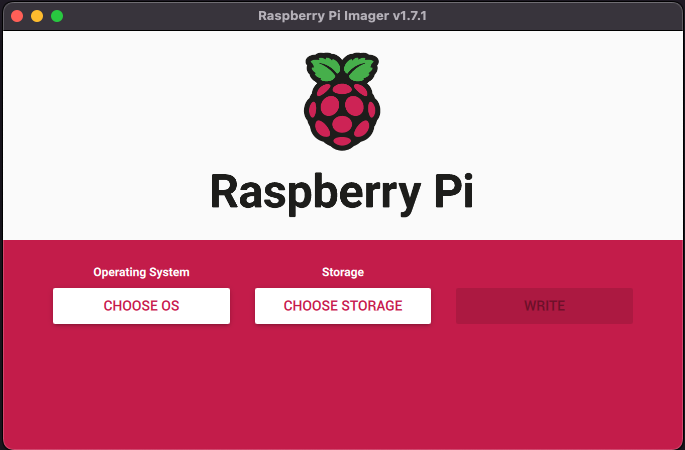
\includegraphics[scale=0.35]{Images/raspberry_pi/app.png}
					\vspace{2mm}
				\end{minipage}
			\item[\textbf{Step 4:}] Click on ``CHOOSE OS'' and Select \textbf{``Raspberry Pi OS (32-bit) Desktop''}\\
				\begin{minipage}{\textwidth}
					\vspace{2mm}
					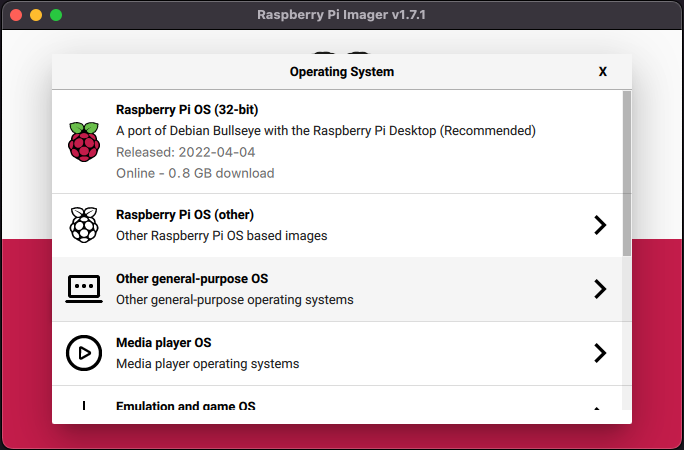
\includegraphics[scale=0.35]{Images/raspberry_pi/choose-os.png}
					\vspace{2mm}
				\end{minipage}
			\item[\textbf{Step 5:}] Click on ``CHOOSE STORAGE'' (\textbf{NOTE:} Please make sure you select correct SD card with is in Raspberry Pi 4)
			\item[\textbf{Step 6:}] Click on ``WRITE''
			\item[\textbf{Step 7:}] Wait untill writting is complete.
		\end{itemize}
	
	\subsection{Login to Raspberry Pi OS}
		At the begining  the user name of the OS is \textbf{``pi''} and password is \textbf{``raspberry''}. (\textbf{NOTE:} For this project we did \textbf{NOT} change any default user and password.)
	
	\subsubsection{Accessing Raspberry Pi}	\label{subsubsec:ssh}
		There are multiple ways you can access the \textbf{``pi''} user.  
		\begin{itemize}[leftmargin=1.2cm]
			\item Accessing through SSH \\
				To access \textbf{``pi''} user using SSH connection you need to make sure that your computer and Raspberry Pi are in same Internet connection. In this project it is ``eduroam'' connection. To setup ``eduroam'' connection into your newly install Raspberry Pi OS, please follow the instruction from \hyperref[sec:run-eduroam]{Section \ref{sec:run-eduroam}}.
				\begin{itemize}[leftmargin=1.3cm]
					\item[\textbf{Step 1:}] Open Terminal in your local computer \\
						\begin{minipage}{\textwidth}
							\vspace{2mm}
							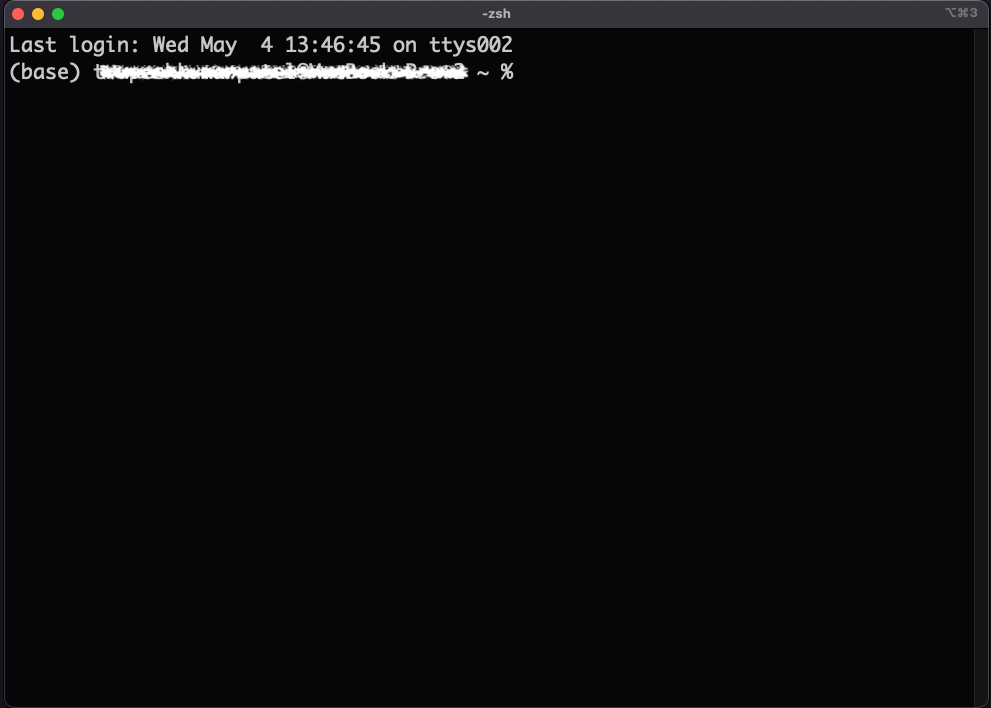
\includegraphics[scale=0.35]{Images/raspberry_pi/ssh_login/open_iterm.png}
							\vspace{2mm}
						\end{minipage}
					\item[\textbf{Step 2:}] Type command ``ssh pi@10.127.227.112'' <-- here `10.127.227.112' is IP address of Raspberry Pi, in your case might be different.\\
						\begin{minipage}{\textwidth}
							\vspace{2mm}
							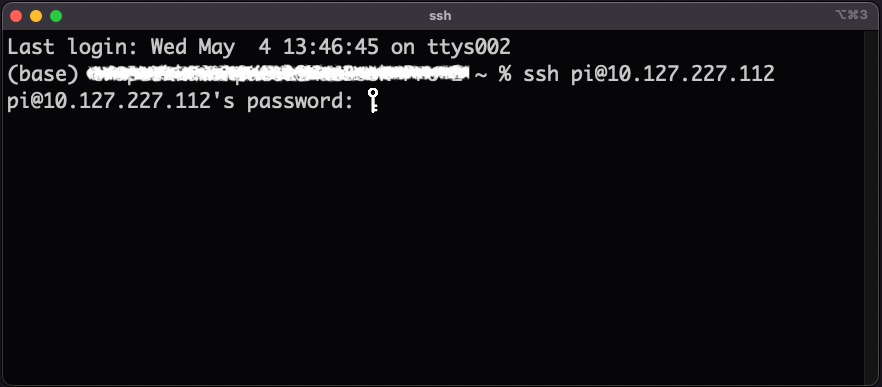
\includegraphics[scale=0.35]{Images/raspberry_pi/ssh_login/login.png}
							\vspace{2mm}
						\end{minipage}
					\item[\textbf{Step 3:}] Enter the password ``raspberry''. Please enter the password that you set if you have, else it is going to be same as the authors.\\
						\begin{minipage}{\textwidth}
							\vspace{2mm}
							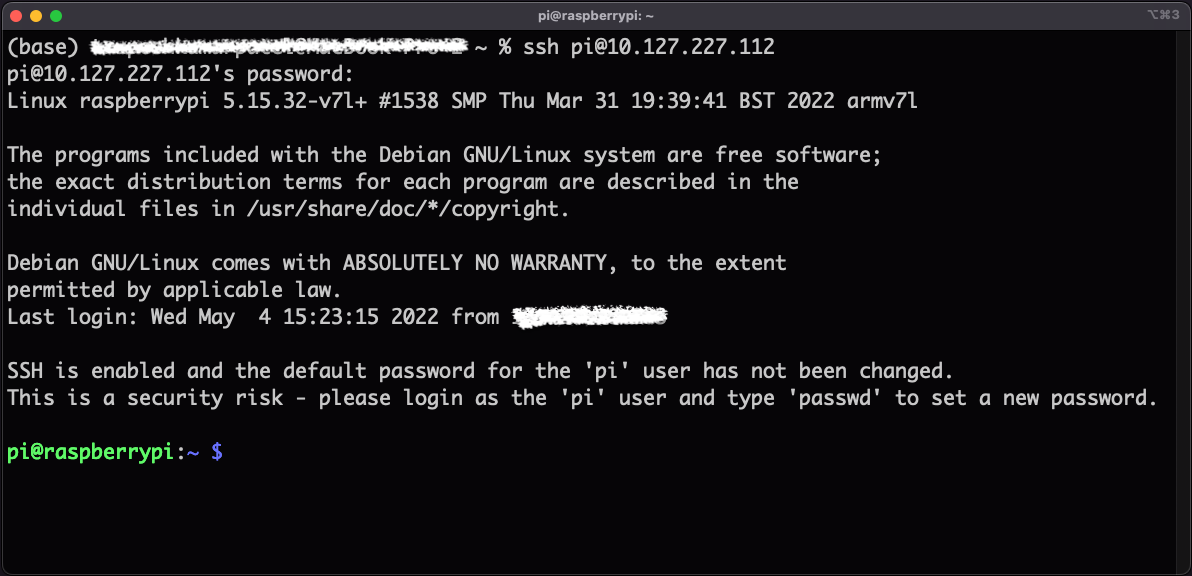
\includegraphics[scale=0.35]{Images/raspberry_pi/ssh_login/after_login.png}
							\vspace{2mm}
						\end{minipage}
				\end{itemize}
		\end{itemize}
	
	\section{Connect to eduroam}	\label{sec:run-eduroam}
	 To re-run the project, you have to connect your Raspberry Pi with ``eduroam'' network at The Univeristy of Alabama. Now, if you have freshly install the Raspberry Pi OS, then you need to run the script called \textbf{``config\_eduroam.sh''}, which can be found \href{https://github.com/TrupeshKumarPatel/IoT_RaspberryPi/tree/main/source_code/eduroam_config}{here}. 
	 
\subsection{Configure Raspberry Pi for eduroam}
		\begin{itemize}[leftmargin=1.8cm]
			\item[\textbf{Step 1:}] Login to the Raspberry Pi as user ``pi'' %(\textbf{Note:} You can follow steps from \hyperref[subsubsec:ssh]{Section \ref{subsubsec:ssh}}.)
			\item[\textbf{Step 2:}] Type command ``{\fontfamily{cmtt}\selectfont{git clone https://github\\.com/TrupeshKumarPatel/IoT\_RaspberryPi.\\git}}''\\
				\begin{minipage}{\textwidth}
					\vspace{2mm}
					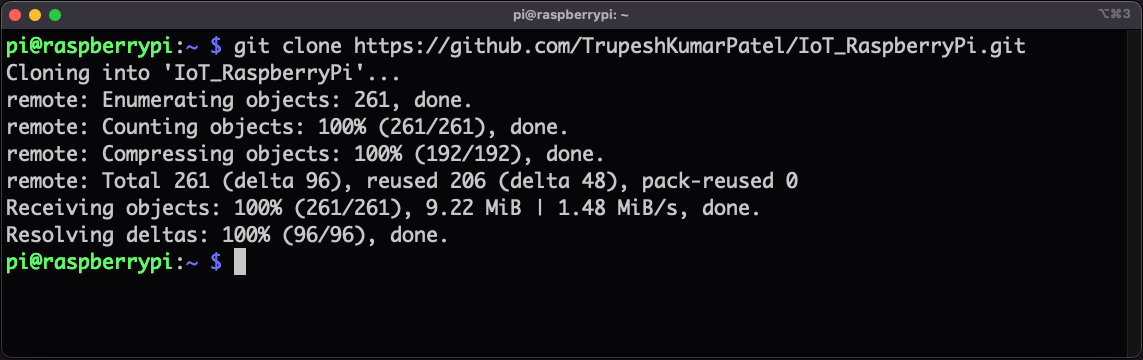
\includegraphics[scale=0.17]{Images/raspberry_pi/eduroam_config/clone_git.png}
					\vspace{2mm}
				\end{minipage}
			\item[\textbf{Step 3:}] Type command ``{\fontfamily{cmtt}\selectfont{sudo su}}'' ~\danger\textbf{NOTE} ~This com\\mand to get sudo access to Raspberry Pi \danger\\
				\begin{minipage}{\textwidth}
					\vspace{2mm}
					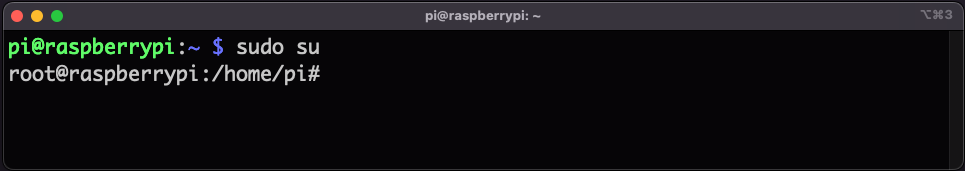
\includegraphics[scale=0.2]{Images/raspberry_pi/eduroam_config/sudo_login.png}
					\vspace{2mm}
				\end{minipage}
			\item[\textbf{Step 4:}] Type command ``{\fontfamily{cmtt}\selectfont{chmod +x IoT\_Raspberry\\Pi/source\_code/eduroam\_config/config\\\_eduroam.sh}}''\\
				\begin{minipage}{\textwidth}
					\vspace{2mm}
					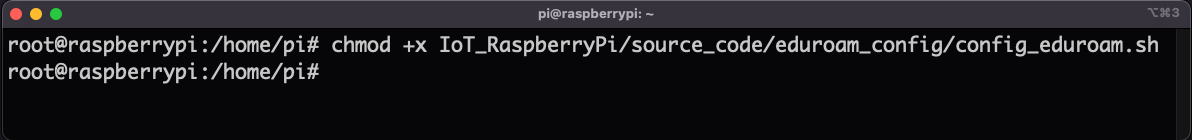
\includegraphics[scale=0.16]{Images/raspberry_pi/eduroam_config/permission_x.png}
					\vspace{2mm}
				\end{minipage}
			\item[\textbf{Step 5:}] Type command ``{\fontfamily{cmtt}\selectfont{./IoT\_RaspberryPi/sourc\\e\_code/eduroam\_c\\onfig/config\_eduroam.sh}}''
			\item[\textbf{Step 6:}] Enter your crimson email address
			\item[\textbf{Step 7:}] Enter your crimson password\\
				\begin{minipage}{\textwidth}
					\vspace{2mm}
					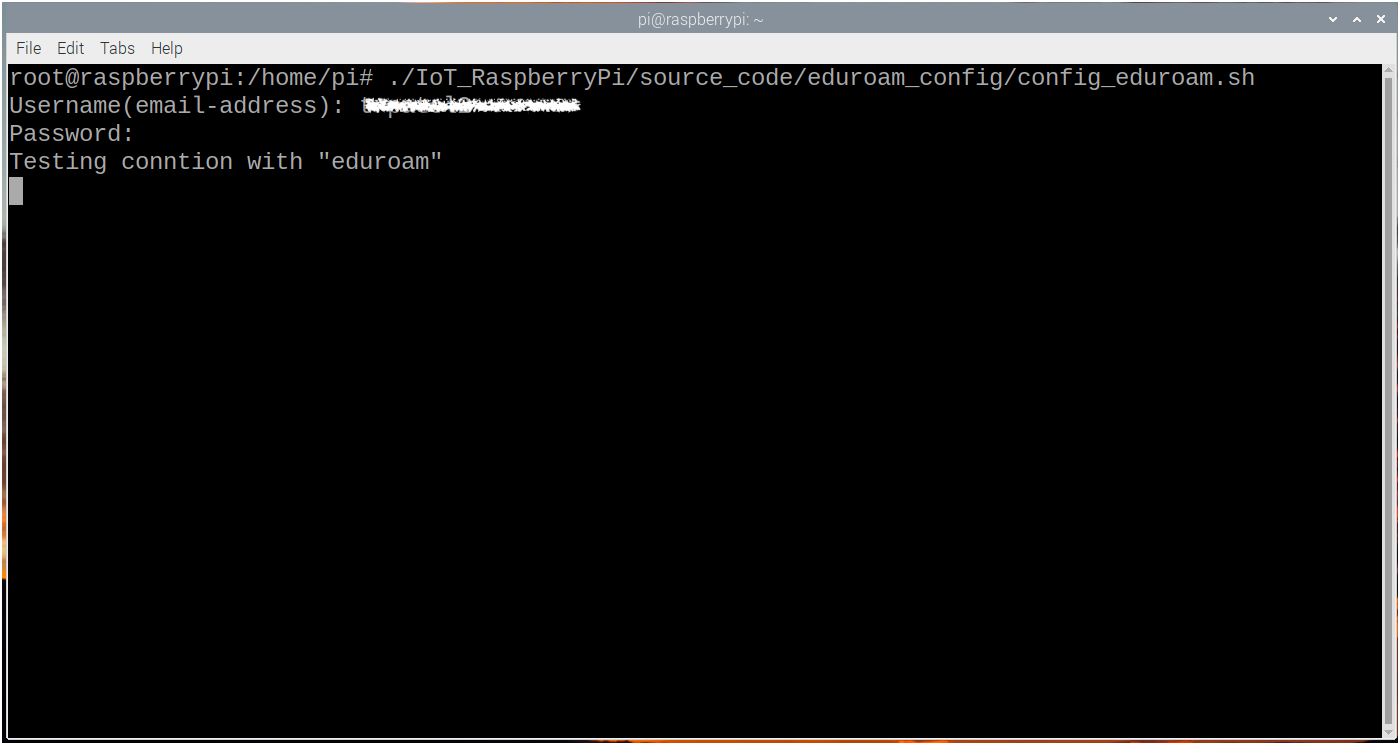
\includegraphics[scale=0.14]{Images/raspberry_pi/eduroam_config/run_eduroam_conf.png}
					\vspace{2mm}
				\end{minipage}
			\item[\textbf{Step 8:}] Now wait for your Raspberry Pi to restart
		\end{itemize}
	
	\section{Installation of Asterisk}	\label{sec:run-asterisk}
	To install Asterisk same as this project authors, please follow below instructions: (\textbf{Note:} Here author installing Asterisk from source code. You can also follow the installation video from \href{https://www.youtube.com/watch?v=52sEPVPV9JE&list=PLruX0IBTg1G4Auvo5YhoJKgskmMP7b8bJ&index=4&ab_channel=InnovateAsterisk}{InnovationAsterisk})
	
	\subsection{Asterisk Installation from the Source Code}
		\begin{itemize}[leftmargin=1.7cm]
			\item[\textbf{Step 1:}] Type command ``{\fontfamily{cmtt}\selectfont{wget http://downloads.asterisk.org/pub/telephony/asterisk/asterisk-18-curren\\t.tar.gz}}''\\
				\begin{minipage}{\textwidth}
					\vspace{2mm}
					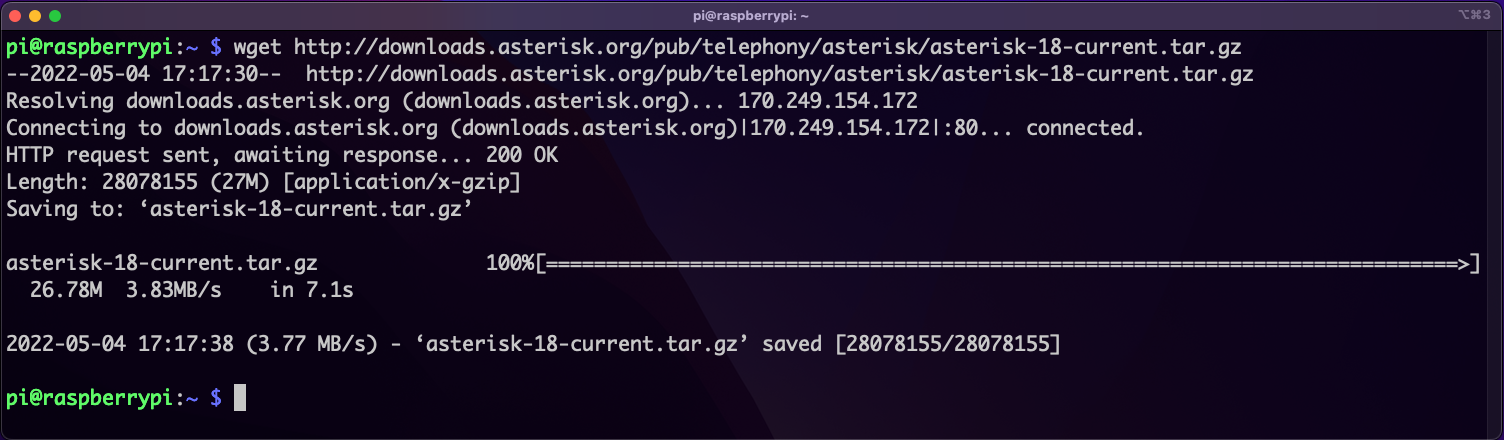
\includegraphics[scale=0.3]{Images/raspberry_pi/asterisk_install/wget.png}
					\vspace{2mm}
				\end{minipage}
			
			\item[\textbf{Step 2:}] Type command ``{\fontfamily{cmtt}\selectfont{sudo apt-get update}}''
			\item[\textbf{Step 3:}] Type command ``{\fontfamily{cmtt}\selectfont{sudo apt-get upgrade}}''
			\item[\textbf{Step 4:}] Type command ``{\fontfamily{cmtt}\selectfont{sudo apt-get install ntp}}''
			\item[\textbf{Step 5:}] Type command ``{\fontfamily{cmtt}\selectfont{sudo apt-get install speex speex* libspeex-dev libspeexdsp-dev}}''
			\item[\textbf{Step 6:}] Type command ``{\fontfamily{cmtt}\selectfont{sudo apt-get install libspeex-dev libspeexdsp-dev speex speex-doc}}''
			\item[\textbf{Step 7:}] Type command ``{\fontfamily{cmtt}\selectfont{sudo apt-get install xmlstarlet libopus-dev libopusfile-dev}}'' <-- (\textbf{NOTE:} This optional if you don't want browser-base telephony, here author did not do this)
			
			\item[\textbf{Step 8:}] Type command ``{\fontfamily{cmtt}\selectfont{tar -xvf asterisk-18-current.tar.gz}}'' <-- This command will extract all the source file into folder called ``asterisk-18.x.x'' (\textbf{Note:} here `x' could be any number based of current relese/download)
			
			\item[\textbf{Step 9:}] Type command ``{\fontfamily{cmtt}\selectfont{cd asterisk-18.x.x}}'' <-- (\textbf{Note:} here `x' could be any number based of current relese/download)
			
			\item[\textbf{Step 10:}] Type command ``{\fontfamily{cmtt}\selectfont{sudo contrib/scripts/install\_prereq install}}'' <-- This will check all the prerequisites of Asterisk. This command will ask few promps to set configurations
					\begin{enumerate}
						\item Telephone code : Type ``{\fontfamily{cmtt}\selectfont{1}}'' for US
					\end{enumerate}
			\item[\textbf{Step 11:}] Type command ``{\fontfamily{cmtt}\selectfont{sudo ./configure --libdir=/usr/lib --with-pjproject-bundled}}''
			
			\item[\textbf{Step 12:}] Type command ``{\fontfamily{cmtt}\selectfont{sudo make menuselect}}'' <-- Please watch this \href{https://www.youtube.com/watch?v=52sEPVPV9JE&list=PLruX0IBTg1G4Auvo5YhoJKgskmMP7b8bJ&index=4&ab_channel=InnovateAsterisk}{video}) from InnovateAsterisk for more details.

			\item[\textbf{Step 13:}] Type command ``{\fontfamily{cmtt}\selectfont{sudo make}}''
			\item[\textbf{Step 14:}] Type command ``{\fontfamily{cmtt}\selectfont{sudo make install}}''
			\item[\textbf{Step 15:}] Type command ``{\fontfamily{cmtt}\selectfont{sudo make samples}}'' <-- This will create all default Asterisk configuration files\\\\
			\danger\textbf{NOTE:} \textbf{Step 16-17} is only required if you haven't downloaded ``IoT\_RaspberryPi'' GitHub repository from \href{https://github.com/TrupeshKumarPatel/IoT_RaspberryPi}{here}  \danger\\
			\item[\textbf{Step 16\danger:}] Type command ``{\fontfamily{cmtt}\selectfont{cd ~}}''
			\item[\textbf{Step 17\danger:}] Type command ``{\fontfamily{cmtt}\selectfont{git clone https://github.com/TrupeshKumarPatel/IoT\_RaspberryPi.git}}''\\
				\begin{minipage}{\textwidth}
					\vspace{2mm}
					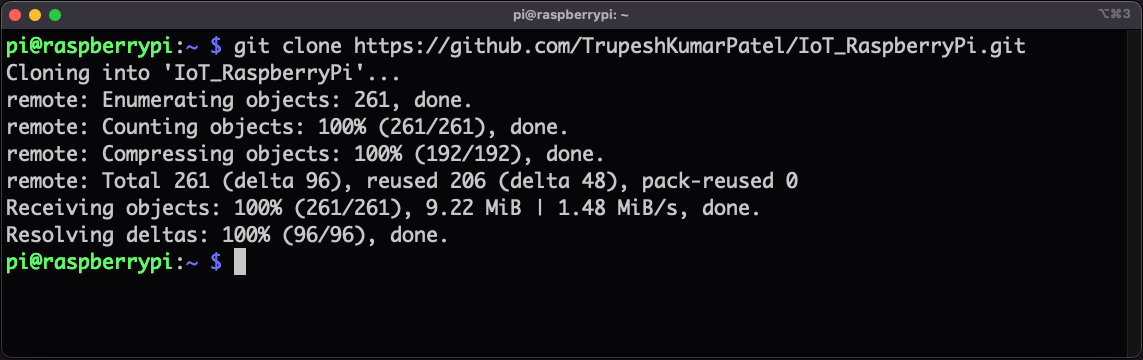
\includegraphics[scale=0.35]{Images/raspberry_pi/eduroam_config/clone_git.png}
					\vspace{2mm}
				\end{minipage}
			\item[\textbf{Step 18:}] Types command ``{\fontfamily{cmtt}\selectfont{sudo cp -R ~/IoT\_RaspberryPi/source\_code/asterisk\_config/* /etc/asterisk/}}''
		\end{itemize}

\pagebreak
\section{Command of Asterisk}	\label{sec:command-asterisk}
	Now, after following instruction from \hyperref[sec:run-asterisk]{Section \ref{sec:run-asterisk}}, you should be able to run asterisk commands.
	\begin{itemize}
		\item To check the status of Asterisk\\
		Type command ``{\fontfamily{cmtt}\selectfont{sudo service asterisk status}}''
		\item To start the Asterisk\\
		Type command ``{\fontfamily{cmtt}\selectfont{sudo service asterisk start}}''
		\item To restart the Asterisk\\
		Type command ``{\fontfamily{cmtt}\selectfont{sudo service asterisk restart}}''
		\item To stop the Asterisk\\
		Type command ``{\fontfamily{cmtt}\selectfont{sudo service asterisk stop}}''
		\item To access CLI of the Asterisk\\
		Type command ``{\fontfamily{cmtt}\selectfont{sudo asterisk -r}}''\\
			\begin{minipage}{\textwidth}
				\vspace{2mm}
				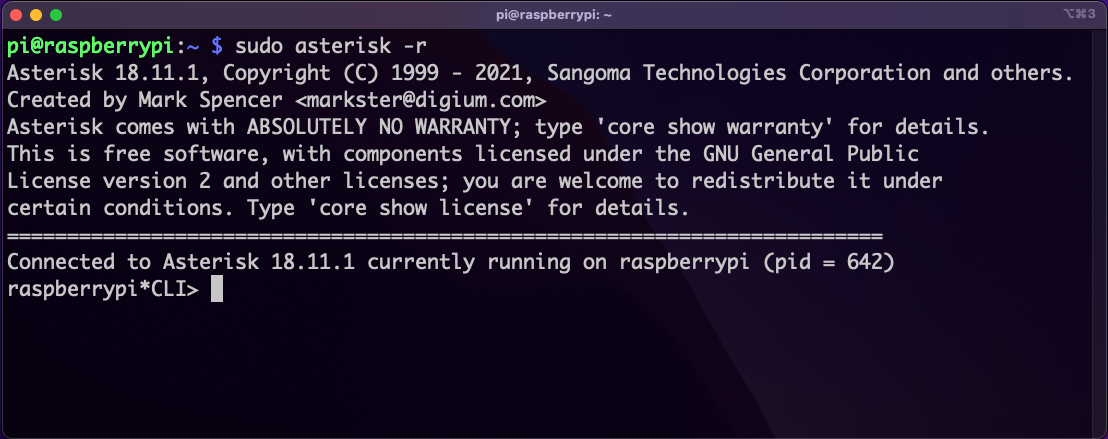
\includegraphics[scale=0.35]{Images/raspberry_pi/asterisk_install/CLI.png}
				\vspace{2mm}
			\end{minipage}
		\item To see all peers\\
		Type command ``{\fontfamily{cmtt}\selectfont{sip show peers}}''\\
			\begin{minipage}{\textwidth}
				\vspace{2mm}
				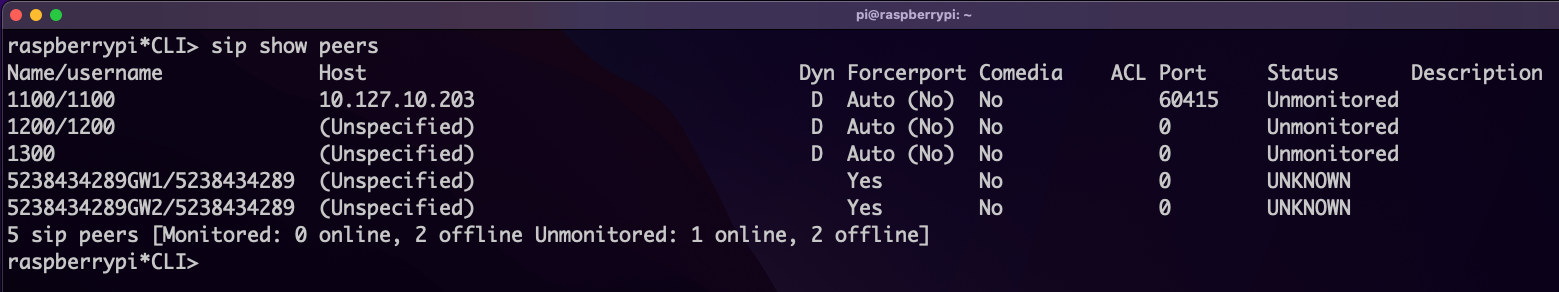
\includegraphics[scale=0.3]{Images/raspberry_pi/asterisk_install/show_peers.png}
				\vspace{2mm}
			\end{minipage}
		\item To see all users\\
		Type command ``{\fontfamily{cmtt}\selectfont{sip show users}}''\\
		\begin{minipage}{\textwidth}
			\vspace{2mm}
			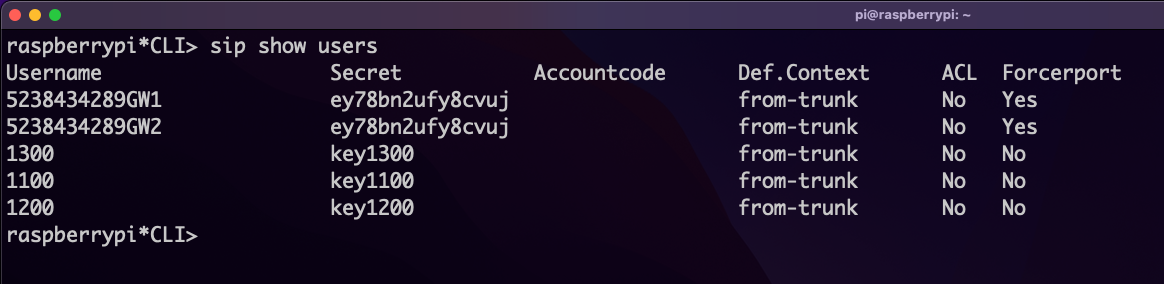
\includegraphics[scale=0.3]{Images/raspberry_pi/asterisk_install/show_users.png}
			\vspace{2mm}
		\end{minipage}
	\end{itemize}
	
	There are many Asterisk commands are available in their document offical website \href{https://wiki.asterisk.org/wiki/display/AST/Asterisk+18+Documentation}{here} and external soure \href{https://www.voip-info.org/asterisk-cli/}{here}, use it as you need.
\end{document}